\documentclass[twoside,11pt]{homework}

\coursename{COMS 4771 Machine Learning (Spring 2020)} 

\studname{Joseph High}    % YOUR NAME GOES HERE
\studmail{jph2185@columbia.edu}% YOUR UNI GOES HERE
\hwNo{5}                   % THE HOMEWORK NUMBER GOES HERE
\date{\today} % DATE GOES HERE

% Uncomment the next line if you want to use \includegraphics.
%\usepackage{graphicx}
\usepackage{graphicx}
%\usepackage{fancyhdr}
\usepackage{enumerate}
\usepackage{amsmath}
\usepackage{relsize}
\usepackage{mathtools}
\usepackage{xfrac}
\usepackage{dsfont}
\usepackage[dvipsnames]{xcolor}
\usepackage[makeroom]{cancel}
\usepackage{collectbox}
\usepackage{placeins}
%\usepackage{cleveref}
\usepackage{eqnarray}
%\usepackage{titlesec} 
\usepackage{bm} 
\usepackage{bbm}
\usepackage{hyperref}
\usepackage{flafter}
\usepackage{graphicx}
\usepackage{float}
\usepackage{algorithm}
\usepackage{algorithmicx}
\usepackage{algpseudocode}
\usepackage{subfig}
%\titleformat{\subsubsection}[runin]
%  {\normalfont\normalsize\bfseries}{\thesubsubsection}{1em}{}

%Euclidean 2-norm:
\DeclarePairedDelimiter{\2norm}{\lVert}{\rVert^2_2}

\newcommand{\defeq}{\vcentcolon=}
\newcommand\unif{\ensuremath{\operatorname{unif}}}

%Expected Value:
\DeclareMathOperator{\EX}{\mathbb{E}}% expected value
\newcommand{\1}[1]{\mathds{1}\left[#1\right]}

% infinity norm:
\DeclarePairedDelimiter{\infnorm}{\lVert}{\rVert_{\infty}}

%Absolute Value:
\DeclarePairedDelimiter\abs{\lvert}{\rvert}

% Regular Euclidean norm (no subscript or exponent):
\DeclarePairedDelimiter{\norm}{\lVert}{\rVert}

\newcommand{\expect}{\operatorname{\mathbb{E}}\expectarg}
\DeclarePairedDelimiterX{\expectarg}[1]{[}{]}{%
  \ifnum\currentgrouptype=16 \else\begingroup\fi
  \activatebar#1
  \ifnum\currentgrouptype=16 \else\endgroup\fi
}

\newcommand{\expectpi}{\operatorname{\mathbb{E}_{\pi}}\expectpiarg}
\DeclarePairedDelimiterX{\expectpiarg}[1]{[}{]}{%
  \ifnum\currentgrouptype=16 \else\begingroup\fi
  \activatebar#1
  \ifnum\currentgrouptype=16 \else\endgroup\fi
}

\newcommand{\innermid}{\nonscript\;\delimsize\vert\nonscript\;}
\newcommand{\activatebar}{%
  \begingroup\lccode`\~=`\|
  \lowercase{\endgroup\let~}\innermid 
  \mathcode`|=\string"8000
}


\makeatletter
\newcommand{\mybox}{%
    \collectbox{%
        \setlength{\fboxsep}{1pt}%
        \fbox{\BOXCONTENT}%
    }%
}


%%%%%%%%%%%%%%%% Direct Comments %%%%%%%%%%%%%%%%
\newcommand{\joe}[1]{\textcolor{black}{\colorbox{cyan}{\parbox{15.5cm}{\textbf{\textsc{Joe}:  #1}}}}}
%newcommand{\joe}[1]{}
%%%%%%%%%%%%%%%%%%%%%%%%%%%%%%%%%%%%%%%%%%


\begin{document}
\maketitle

\section*{Problem 1: Improving the Confidence}

\begin{proof}
Using the hint, one can construct an algorithm (referred to as algorithm $\mathcal{B}$, or just $\mathcal{B}$, henceforth) that calls algorithm $\mathcal{A}$ on $k$ independent sets of training samples where each run will be done over a draw of $n = O\left(\frac{1}{\epsilon^2}\right)$ samples. In total, $\mathcal{B}$ is run over a draw of $n'$ samples such that the error of the resulting model is within $\epsilon$-distance of the model with minimum error over all $f \in \mathcal{F}$. Algorithm $\mathcal{B}$ is constructed below.\\\ \\\
%
Fix an $ \ \mathlarger{\epsilon_1 = \frac{\epsilon}{2}} \ $ such that with probability $0.55$ we have the following for each run of $\mathcal{A}$\\[0.3em] (over a draw of $n$ samples in each run): 

\begin{align}\label{ineq1}
\text{err}(f_n^{\mathcal{A}}) - \inf_{f \in \mathcal{F}}\text{err}(f) \ \leq \ \epsilon_1 \ \ \ 
\Longleftrightarrow \ \ \ \text{err}(f_n^{\mathcal{A}}) \ \leq \ \inf_{f \in \mathcal{F}}\text{err}(f) + \epsilon_1 
\end{align}


\noindent
Fix a $\delta > 0$ and choose some $\gamma_1 \leq \frac{\delta}{2}$ \ such that with probability $1- \gamma_1 \ \geq \ 1 - \frac{\delta}{2} \ $ $\left(\right.$i.e., with probability at least $\left.  1 - \frac{\delta}{2}\right)$, the $k$ iterations of algorithm $\mathcal{A}$ will return at least one model with a generalization error within $\frac{\epsilon}{2}$  of $ \ \mathlarger{\inf_{f \in \mathcal{F}}\text{err}(f)}$. Henceforth, such a model will be referred to as a ``good" model, while models that don't exhibit this behavior will be referred to as ``bad". Let $\mathcal{F_{\mathcal{B}}}$ be the collection of the $k$ models returned by algorithm $\mathcal{A}$. That is, for $i \in \{1, \dots, k\}$, let $f^{\mathcal{A}}_{n_i}$ denote the model returned by $\mathcal{A}$ in the $i^{th}$ run, then $\mathcal{F_{\mathcal{B}}} = \left\lbrace f^{\mathcal{A}}_{n_1}, \dots, f^{\mathcal{A}}_{n_k} \right\rbrace$. The number of models in $\mathcal{F_{\mathcal{B}}}$ (i.e., the number of iterations of $\mathcal{A}$) should be sufficiently large so that the probability of at least one ``good" model being returned is at least $1 - \frac{\delta}{2}$. To determine a sufficient $k$, consider the following:\\\ 
Let $E_i$ be the random variable that denotes the event that the $i^{th}$ model, $f^{\mathcal{A}}_{n_i}$, is a ``good" model. That is, let $E_i = \left\lbrace \text{err}\left( f^{\mathcal{A}}_{n_i} \right) - \inf_{f \in \mathcal{F}}\text{err}\left(f \right) \ \leq \ \frac{\epsilon}{2} \right\rbrace$. Then, the complement, $E_i^{\mathrm{c}}$, is the event that $f^{\mathcal{A}}_{n_i}$ is a ``bad" model: $E_i^{\mathrm{c}} = \left\lbrace \text{err}\left( f^{\mathcal{A}}_{n_i} \right) - \inf_{f \in \mathcal{F}}\text{err}\left(f \right) \ > \ \frac{\epsilon}{2} \right\rbrace$. From the supposition, the probability that the $i^{th}$ run of $\mathcal{A}$ returns a ``bad" model is
$$\mathbb{P}\left( E_i^{\mathrm{c}} \right) = 1 - \mathbb{P}\left(E_i\right) = 1 - 0.55 = 0.45$$
Then, the probability that all $k$ models returned by $\mathcal{A}$ are ``bad" is
\begin{align*}
\mathbb{P}\left(\forall i \in \{1, \dots, k\} : \ f^{\mathcal{A}}_{n_i} \in \mathcal{F}_{\mathcal{B}} \text{ is ``bad"}\right) \ &= \ \mathbb{P}\left( \bigcap_{i=i}^k E_i^{\mathrm{c}} \right) \ = \ \prod_{i=1}^k \mathbb{P}\left( E_i^{\mathrm{c}} \right) = \prod_{i=1}^k 0.45 = (0.45)^k
\intertext{Then, the probability that there is \textit{at least one} ``good" model in $\mathcal{F}_{\mathcal{B}}$ is}
\mathbb{P}\left(\exists  i \in \{1, \dots, k\} : \ f^{\mathcal{A}}_{n_i} \in \mathcal{F}_{\mathcal{B}} \text{ is ``good"}\right) \ &= \ 1 - \mathbb{P}\left( \bigcap_{i=i}^k E_i^{\mathrm{c}} \right) \ = \ 1 - (0.45)^k 
\end{align*}
Therefore, we need to choose a $k$ such that
\begin{align*}
& 1 - (0.45)^k \ \geq \ 1 - \frac{\delta}{2} \ \ \ \Longleftrightarrow \ \ \ (0.45)^k \ \leq \ \frac{\delta}{2}
\ \ \ \Longleftrightarrow \ \ \ k\ln(0.45) \ \leq \ \ln\left(\frac{\delta}{2}\right)\\[0.5em]
& \Longleftrightarrow \ \ \ -k\ln\left(\frac{1}{0.45}\right) \ \leq \ -\ln\left(\frac{2}{\delta}\right) \ \ \ \Longleftrightarrow \ \ \ k \ \geq \ \frac{\ln\left(\frac{2}{\delta}\right)}{\ln\left(\frac{1}{0.45}\right)}
%\intertext{Since $k$ is necessarily an integer, the ceiling function is applied to the right-hand %side of the last inequality:}
%k \ = \ \left\lceil\frac{\ln\left(\frac{2}{\delta}\right)}{\ln\left(\frac{1}{0.45}\right)}\right\rceil
\end{align*}
\\\

%To determine a sufficient $k$, let $X_i \in \{0, 1\}$ be a r.v. that takes on denotes the number of ``good" models that are returned in the $k$ iterations of $\mathcal{A}$. Then, the probability that at least one ``good" model is returned is
%\begin{align*}
%P(X \geq 1) = \sum_{x = 1}^k  (1-0.55)^{k-1}(0.55) \ & = \ (0.55)\sum_{x = 1}^k  (0.45)^{k-1} \\[0.5em]
%& = \ (0.55)\sum_{x = 0}^{k-1}  (0.45)^{k} \\[0.5em]
%& = \ (0.55)\left(\frac{1 - (0.45)^k}{1 - 0.45}\right) \\[0.5em]
%& = \ 1 - (0.45)^k
%\end{align*}
%Therefore, we need to choose a $k$ such that
%\begin{align*}
%& 1 - (0.45)^k \ \geq \ 1 - \frac{\delta}{2} \ \ \ \Longleftrightarrow \ \ \ (0.45)^k \ \leq \ \frac{\delta}{2}
%\ \ \ \Longleftrightarrow \ \ \ k\ln(0.45) \ \leq \ \ln\left(\frac{\delta}{2}\right)\\[0.5em]
%& \Longleftrightarrow \ \ \ -k\ln\left(\frac{1}{0.45}\right) \ \leq \ -\ln\left(\frac{2}{\delta}\right) \ \ \ \Longleftrightarrow \ \ \ k \ \geq \ \frac{\ln\left(\frac{2}{\delta}\right)}{\ln\left(\frac{1}{0.45}\right)}
%%\intertext{Since $k$ is necessarily an integer, the ceiling function is applied to the right-hand %side of the last inequality:}
%%k \ = \ \left\lceil\frac{\ln\left(\frac{2}{\delta}\right)}{\ln\left(\frac{1}{0.45}\right)}\right\rceil
%\end{align*}
\noindent
%While this holds for $\forall k  \geq  \frac{\ln\left(\sfrac{2}{\delta}\right)}{\ln\left(\sfrac{1}{0.45}\right)}$, 
It suffices to set $k  = \left\lceil\frac{\ln\left(\sfrac{2}{\delta}\right)}{\ln\left(\sfrac{1}{0.45}\right)}\right\rceil$. Indeed, $k$ is necessarily an integer, so the ceiling function should be applied to the right-hand side. %That is, the number of times that $\mathcal{B}$ calls $\mathcal{A}$ should be such that $k \ \geq \ \left\lceil\frac{\ln\left(\frac{2}{\delta}\right)}{\ln\left(\frac{1}{0.45}\right)}\right\rceil$.
\\\ \\\
%Let $\mathcal{F_{\mathcal{B}}}$ be the collection of the $k$ models returned by algorithm $\mathcal{A}$. 
Since $\mathcal{F_{\mathcal{B}}}$ is finite, the ERM algorithm can be applied to $\mathcal{F_{\mathcal{B}}}$. Then, for a fixed confidence level $\gamma_2 \leq \frac{\delta}{2}$ and tolerance $\epsilon_2 = \frac{\epsilon}{2}$, apply the ERM algorithm over $\mathcal{F_{\mathcal{B}}}$ using a test set of size $m$. By Occam's Razor, such an $m$ should be such that\footnote{The specific inequality used here was extracted from the proof of efficient PAC learnability for finite $\mathcal{F}$, using the the ERM algorithm, provided in the Learning Theory lecture notes (slide 8).}
$$m \ \geq \ \frac{1}{2\epsilon_2^2}\ln\left(\frac{2|\mathcal{F_{\mathcal{B}}}|}{\gamma_2}\right) \ \geq \ \frac{1}{2(\sfrac{\epsilon}{2})^2}\ln\left(\frac{2k}{\sfrac{\delta}{2}}\right) \ = \ \frac{2}{\epsilon^2}\ln\left(\frac{4k}{\delta}\right)$$ 
\\\
and since $m$ is necessarily a positive integer, we can set $m = \left\lceil\frac{2}{\epsilon^2}\ln\left(\sfrac{4k}{\delta}\right)\right\rceil$.  \\\
Let $f_m^{ERM}$ be the model returned by the ERM algorithm. If follows from Occam's Razor that, with probability at least $1 - \frac{\delta}{2}$, 
\begin{equation}\label{ineq2}
\text{err}\left(f_m^{ERM}\right) - \inf_{f \in \mathcal{F_{\mathcal{B}}}}\text{err}(f) \ \leq \ \epsilon_2
\end{equation}
Now, the probability that algorithm $\mathcal{B}$ fails is equal to the probability that either algorithm $\mathcal{A}$ fails to return a ``good" model in $k$ iterations or the ERM algorithm fails to select a ``good" model from $\mathcal{F}_{\mathcal{B}}$. That is,
\begin{align*}
\mathbb{P}(\mathcal{B} \text{ fails}) \ &= \ \mathbb{P}\left(\left\lbrace \forall f^{\mathcal{A}}_{n_i} \in \mathcal{F}_{\mathcal{B}} \ : \ \text{err}\left(f^{\mathcal{A}}_{n_i}\right) - \inf_{f \in \mathcal{F}}\text{err}(f)  > \epsilon_1\right\rbrace \bigcup  \left\lbrace\text{err}\left(f_m^{ERM}\right) - \inf_{f \in \mathcal{F_{\mathcal{B}}}}\text{err}(f)  > \epsilon_2\right\rbrace \right)\\[0.8em]
& \leq \ \mathbb{P}\left\lbrace \forall f^{\mathcal{A}}_{n_i} \in \mathcal{F}_{\mathcal{B}} \ : \ \text{err}\left(f^{\mathcal{A}}_{n_i}\right) - \inf_{f \in \mathcal{F}}\text{err}(f)  > \epsilon_1\right\rbrace \ + \  \mathbb{P}\left\lbrace\text{err}\left(f_m^{ERM}\right) - \inf_{f \in \mathcal{F_{\mathcal{B}}}}\text{err}(f)  > \epsilon_2\right\rbrace \\[0.8em]
& = \ \gamma_1 \ + \ \gamma_2 \ \leq \ \frac{\delta}{2} \ + \ \frac{\delta}{2} \ = \ \delta
\end{align*}
where the second inquality is a result of Boole's inequality (a.k.a. subadditivity).\\\
Then, by combining inequalities (\ref{ineq1}) and (\ref{ineq2}), we have, with probability at least $1 - \delta$,
\begin{align*}
\text{err}(f_m^{ERM})  \ &\leq \ \epsilon_2 + \inf_{f \in \mathcal{F_{\mathcal{B}}}}\text{err}(f)\\[0.5em]
& \leq \ \epsilon_2 + (\epsilon_1 + \inf_{f \in \mathcal{F}}\text{err}(f)) \\[0.5em]
& = \ \frac{\epsilon}{2} + \frac{\epsilon}{2} + \inf_{f \in \mathcal{F}}\text{err}(f)) \\[0.5em]
\Longrightarrow \ \ \ \ \text{err}(f_m^{ERM}) - \inf_{f \in \mathcal{F}}\text{err}(f)) \ &\leq \ \epsilon
\end{align*}
Since $f_m^{ERM}$ is an arbitrary model returned by algorithm $\mathcal{B}$, the above inequality holds for any model returned by algorithm $\mathcal{B}$, with probability at least $1 - \delta$. Note, each run of algorithm $\mathcal{B}$ is over a draw of $n' = kn + m$ \ samples. Indeed, $k \cdot n$ samples are used for the $k$ iterations of $\mathcal{A}$ and $m$ test samples are used to identify the model in $\mathcal{F}_{\mathcal{B}}$ with the minimum empirical error. Then, denote any model returned by $\mathcal{B}$ as $f_{n'}^{\mathcal{B}}$.  Hence, for a tolerance $\epsilon > 0$, with probability at least $1-\delta$, we have
$$\text{err}(f_{n'}^{\mathcal{B}}) - \inf_{f \in \mathcal{F}}\text{err}(f)) \ \leq \ \epsilon$$

\noindent
Moreover, 
\begin{align*}
k \ &= \ \left\lceil\frac{\ln\left(\sfrac{2}{\delta}\right)}{\ln\left(\sfrac{1}{0.45}\right)}\right\rceil \ \ \ \Longrightarrow \ \ k \ = \ O\left(\ln\left(\sfrac{1}{\delta}\right)\right)\\[1.5em]
m \ &= \ \left\lceil\frac{2}{\epsilon^2}\ln\left(\sfrac{4k}{\delta}\right)\right\rceil \ \ \Longrightarrow \ \ m \ = \ O\left(\frac{1}{\epsilon^2}\ln\left(\sfrac{1}{\delta}\right)\right)
\end{align*}
Recall that, $n \ = \ O\left(\frac{1}{\epsilon^2}\right)$. Therefore, since \ $n' = nk + m \ \ \Longrightarrow \ \ n' \ = \ O\left(\frac{1}{\epsilon^2}\ln\left(\sfrac{1}{\delta}\right)\right)$.\\\
Since \ $\ln\left(\sfrac{1}{\delta}\right)$ grows at a slower rate than $\sfrac{1}{\delta}$ (i.e., $\ln\left(\sfrac{1}{\delta}\right) \leq \sfrac{1}{\delta}$), then $n'$ is bounded by a polynomial in both $\sfrac{1}{\epsilon}$ and $\sfrac{1}{\delta}$. That is, $n' \ = \ O\left(\frac{1}{\epsilon^2}\ln\left(\sfrac{1}{\delta}\right)\right) \in \text{poly}\left(\frac{1}{\epsilon} \ , \ \frac{1}{\delta}\right)$, or equivalently
$$n' = \text{poly}\left(\frac{1}{\epsilon} \ , \ \frac{1}{\delta}\right)$$

\noindent
Hence, $\mathcal{F}$ is \textit{efficiently} PAC-learnable.
%\begin{align*}
%m \ = \ \left\lceil\frac{2}{\epsilon^2}\ln\left(\sfrac{4k}{\delta}\right)\right\rceil \ &= \ \left\lceil\frac{2}{\epsilon^2}\ln\left(\frac{4\left\lceil\frac{\ln\left(\sfrac{2}{\delta}\right)}{\ln\left(\sfrac{1}{0.45}\right)}\right\rceil}{\delta}\right)\right\rceil\\[1em]
%& \leq \ \frac{2}{\epsilon^2}\ln\left(\frac{4\left\lceil\frac{\ln\left(\sfrac{2}{\delta}\right)}{\ln\left(\sfrac{1}{0.45}\right)}\right\rceil}{\delta}\right)\\[1em]
%m \ = \ O\left(\frac{1}{\epsilon^2}\ln\left(\sfrac{1}{\delta}\right)\right)
%\intertext{and recall that}
%n \ &= \ O\left(\frac{1}{\epsilon^2}\right)
%\end{align*}

\end{proof}




\section*{Problem 2: Non-linear Dimensionality Reduction}

\begin{enumerate}[(i)]

\item For some $i \in \{1, \dots, n\}$, the derivative of the objective function with respect to $y_i$ is as follows:
\begin{align*}
\frac{\partial}{\partial y_i}\sum_{i,j}\left(\norm{y_i - y_j} - \pi_{ij}\right)^2 \ &= \ \sum_{i,j}\frac{\partial}{\partial y_i}\left[\left(\norm{y_i - y_j} - \pi_{ij}\right)^2\right]\\[0.7em]
&= \ \sum_{\substack{i, j \\ j\neq i}} 2\left(\norm{y_i - y_j} - \pi_{ij}\right) \cdot \frac{\partial}{\partial y_i}\Big[\norm{y_i - y_j} - \pi_{ij}\Big]\\[0.7em]
%&= \ 2\sum_{\substack{i, j \\ j\neq i}}\left(\norm{y_i - y_j} - \pi_{ij}\right) \cdot \frac{\partial}{\partial y_i}\left(\sqrt{({y_i}_1 - {y_j}_1)^2 + \cdots + ({y_i}_d - {y_j}_d)^2} - \pi_{ij}\right)\\[0.7em]
%&= \ 2\sum_{\substack{i, j \\ j\neq i}}\left(\norm{y_i - y_j} - \pi_{ij}\right) \cdot \frac{1}{2}\left(({y_i}_1 - {y_j}%_1)^2 + \cdots + ({y_i}_d - {y_j}_d)^2\right)^{-\sfrac{1}{2}} \cdot \\[-0.7em]
%&\quad \ \ \ \ \ \ \ \ \ \ \ \ \ \ \ \ \ \ \ \ \ \ \ \ \ \ \ \ \ \ \ \ \ \ \ \ \ \ \ \ \ \ \ \ \ \ \ \cdot 2\left[({y_i}_1 - {y_j}_1) + \cdots + ({y_i}_d - {y_j}_d)\right] \\[0.7em]
&= \ 2\sum_{\substack{i, j \\ j\neq i}}\left(\norm{y_i - y_j} - \pi_{ij}\right) \cdot \frac{y_i - y_j}{\norm{y_i - y_j}}\\[0.7em]
&= \ 2\sum_{\substack{i, j \\ j\neq i}}\left(1 - \frac{\pi_{ij}}{\norm{y_i - y_j}} \right) (y_i - y_j)
\end{align*}


\item The optimization problem is \textit{non-convex}. While the feasible region, $\mathbb{R}^d$, is a convex set (since the problem is unconstrained), the objective function is not a convex function. To see this, consider the following:
$$\sum_{i,j}(\norm{y_i - y_j} - \pi_{ij})^2 \ = \ \sum_{i,j} \norm{y_i - y_j}^2 - 2\pi_{ij}\norm{y_i - y_j} + \pi_{ij}^2$$
Without loss of generality, consider one summand
$$\underbrace{\norm{y_i - y_j}^2}_{\text{convex}} \ - \ \underbrace{2\pi_{ij}\norm{y_i - y_j} + \pi_{ij}^2}_{\text{convex}}$$
Note that all $p$-norms are convex functions, provided that $p \geq 1$. Now, because the $\pi_{ij}$ terms denote the shortest path between data points $x_i$ and $x_j$, they're deterministic scalars, and so each summand is the difference of convex functions, which is the equivalent to the sum of a convex function and a concave function. The difference of convex functions is not necessarily convex, but it could be.

\textit{Counter-example}: Let $f(y_1) = \sum_{i,j}(\norm{y_i - y_j} - \pi_{ij})^2$. Without loss of generality, let $d=1$, that is, $y_j \in \mathbb{R}^1$ and suppose that $n=3$. Fix $y_2 = 0$ and $y_3 = 1$, and suppose $\pi_{12} = \pi_{13} = 1$. The objective is then
$$f(y_1) = \sum_{j=2}^3(\norm{y_i - y_j} - \pi_{1j})^2 = (\norm{y_1} - 1)^2 \ + \ (\norm{y_1 - 1} - 1)^2$$
Recall that a function $g$ is convex if and only if for all $x, y \in \mathbf{dom}(g)$, $$g(y) \geq g(x) + g'(x)(y-x)$$ 

Proceeding with this in mind, consider $f$ at $y_1 = \frac{1}{2}$ and $y_1 = \frac{5}{4}$:
$$f( \sfrac{1}{2}) = (\norm{ \sfrac{1}{2}}-1)^2 \ + \ (\norm{ \sfrac{1}{2} - 1} - 1)^2 = \sfrac{1}{2} $$
$$f( \sfrac{5}{4}) = (\norm{\sfrac{5}{4}}-1)^2 \ + \ (\norm{\sfrac{5}{4} - 1} - 1)^2 = \sfrac{5}{8} $$
The derivative of the objective was computed in part (i), which will be used here to compute $f'(2)$:
$$f'(\sfrac{1}{2}) = 2 \cdot \left[\left(1 - \frac{1}{\norm{\sfrac{1}{2}}}\right)(\sfrac{1}{2})  +  \left(1 - \frac{1}{\norm{\sfrac{1}{2} - 1}}\right)(\sfrac{1}{2}-1)\right] = 2 \cdot(\sfrac{1}{4} - \sfrac{3}{4}) = 0$$
Then, $f(2) + f'(2)\cdot(3-2) = 1 + 2 = 3$



\begin{figure}[H]\centering
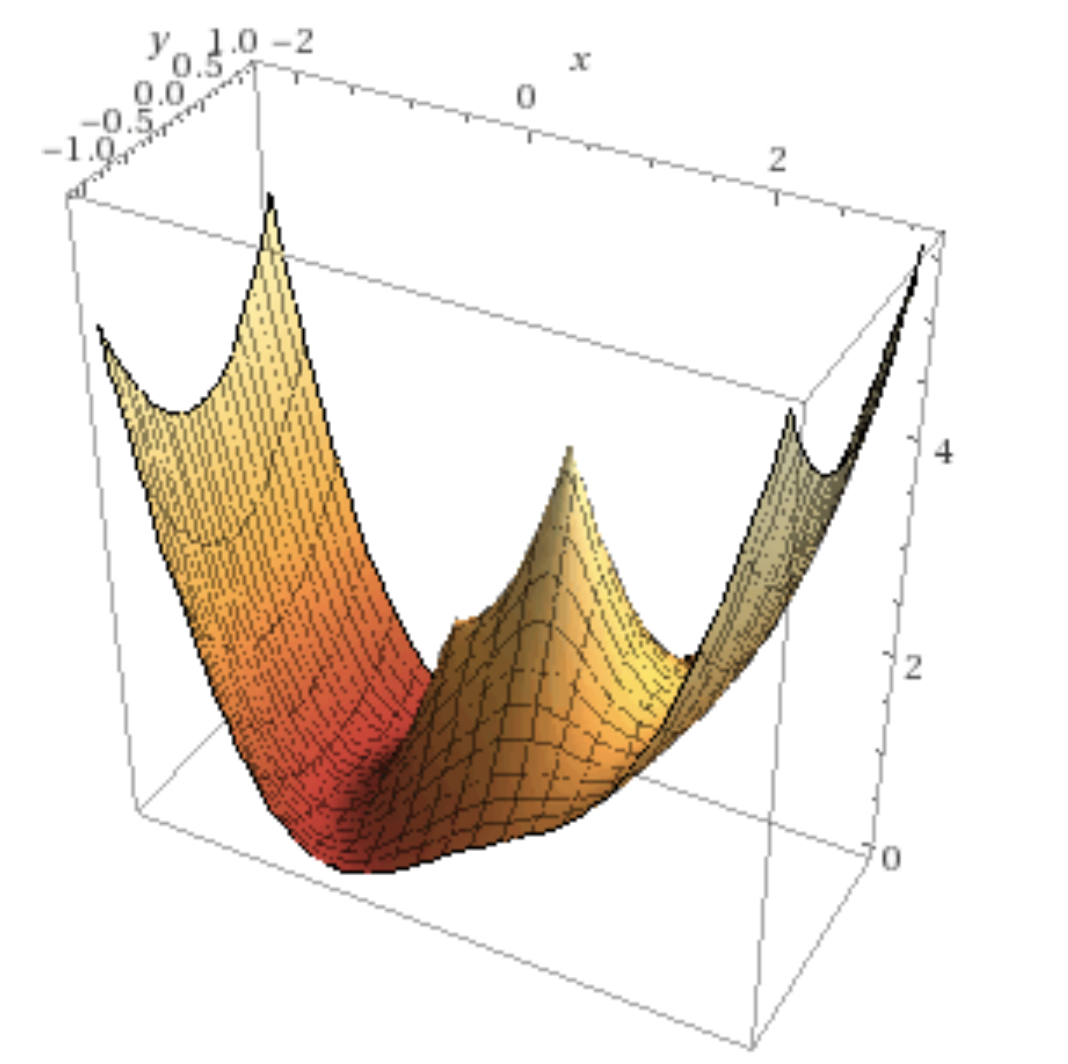
\includegraphics[width=2.5in]{mds}
\end{figure}

\item Code submitted to Courseworks.


\item  Below are the results of PCA on the \texttt{swiss\_roll.txt} data set (implemented in Python).

\textit{Swiss Roll Results} (\texttt{swiss\_roll.txt})

\begin{figure}[H]
\centering
\subfloat[3-Dimensional Swiss Roll]{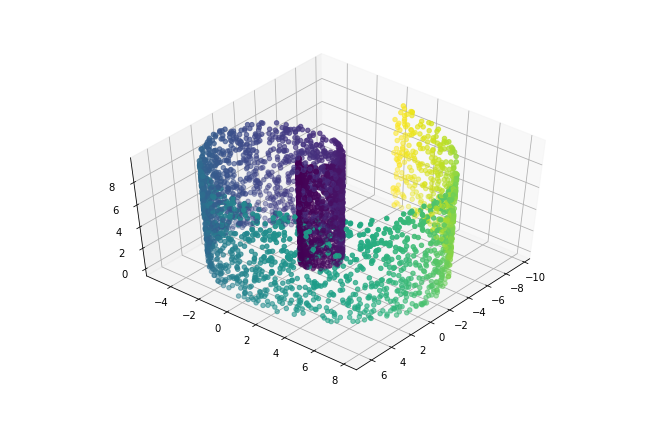
\includegraphics[width=4in]{../code/swiss_3d}}
\subfloat[PCA Embedding]{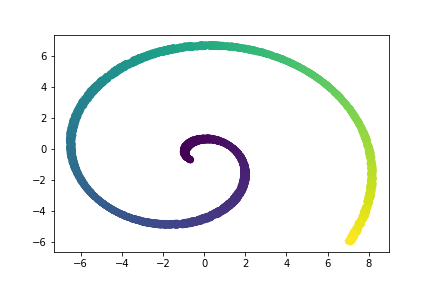
\includegraphics[width=3.5in]{../code/swiss_pca}}
\noindent
\end{figure}


Below are the results of my implementation of the non-linear embedding algorithm given in the homework on the \texttt{swiss\_roll.txt} data set. The non-linear embedding succeeded and appears to have done far better than PCA.

\begin{figure}[H]
\centering
\caption{Low-Dimensional Embedding Result (\texttt{swiss\_roll.txt})}
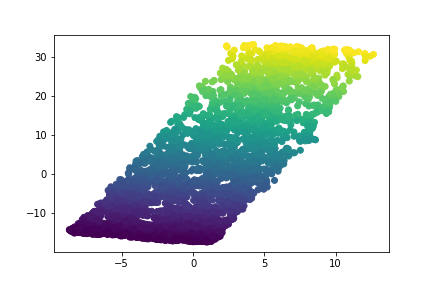
\includegraphics[width=3.5in]{../code/2d_embedding}
\end{figure}

\textit{Swiss Roll Hole Results} (\texttt{swiss\_roll\_hole.txt})

 Below are the results of PCA on the \texttt{swiss\_roll\_hole.txt} data set (implemented in Python).
 
\begin{figure}[H]
\centering
\subfloat[3-Dimensional Swiss Roll with hole]{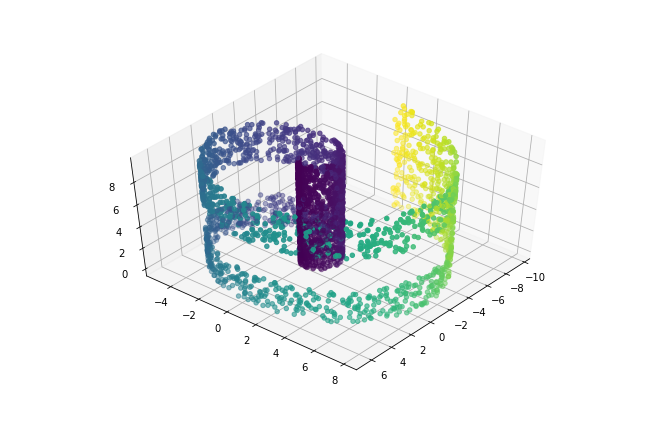
\includegraphics[width=4in]{../code/swiss_hole_3d}}
\subfloat[PCA Embedding of Swiss Roll with hole]{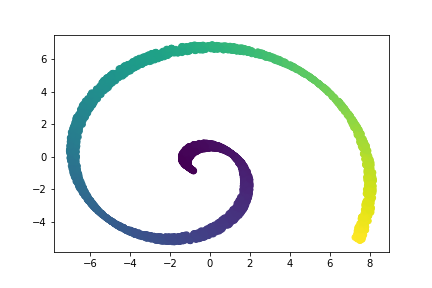
\includegraphics[width=3.5in]{../code/swiss_hole_pca}}
\noindent
\end{figure}


Below are the results of my implementation of the non-linear embedding algorithm given in the homework on the \texttt{swiss\_roll\_hole.txt} data set. Similar to the result for the other data set, the non-linear embedding succeeded and appears to have done far better than PCA.

\begin{figure}[H]
\centering
\caption{Low-Dimensional Embedding Result (\texttt{swiss\_roll\_hole.txt})}
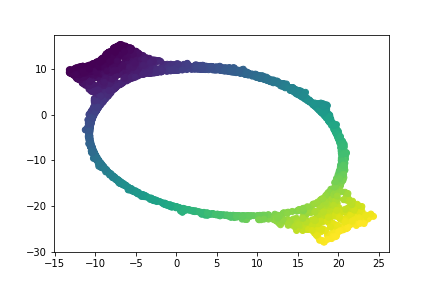
\includegraphics[width=3.5in]{../code/2d_embedding_hole}
\end{figure}


When the learning rate was set at $0.01$, the non-linear embedding failed to capture sufficient information from the  swiss roll. However, when the learning rate was adjusted to $0.0001$, the nonlinear embedding improved,  significantly.
\end{enumerate}


\end{document} 
